\documentclass[conference,onecolumn]{IEEEtran}
\IEEEoverridecommandlockouts
\usepackage[utf8]{inputenc}
\usepackage[T1]{fontenc}
\usepackage{cite}
\usepackage{amsmath,amssymb,amsfonts}
\usepackage{algorithmic}
\usepackage{graphicx}
\usepackage{listings}
\usepackage{float}
\usepackage{textcomp}
\usepackage{gensymb}
\usepackage{xcolor}
\usepackage{url}
\usepackage[spanish,es-noshorthands]{babel}
\def\BibTeX{{\rm B\kern-.05em{\sc i\kern-.025em b}\kern-.08em
    T\kern-.1667em\lower.7ex\hbox{E}\kern-.125emX}}

\lstset{
  basicstyle=\ttfamily\footnotesize,
  keywordstyle=\color{blue},
  commentstyle=\color{gray},
  stringstyle=\color{red},
  frame=single,
  breaklines=true,
  numbers=left,
  numberstyle=\tiny\color{gray}
}

\begin{document}

\title{Co-simulación SUMO + ns-3 (5G-LENA) de una ambulancia inteligente sobre
red 5G NR: mMTC, misión crítica y \textit{network slicing} URLLC/eMBB en un
escenario urbano de Cuenca}

\author{\IEEEauthorblockN{Tyrone Miguel Novillo Bravo}
\IEEEauthorblockA{\textit{Facultad de Ingenier\'ia} \\
\textit{Departamento de Telecomunicaciones}\\
Universidad de Cuenca \\
tyrone.novillo@ucuenca.edu.ec}
\and
\IEEEauthorblockN{Freddy Eduardo L\'opez Padilla}
\IEEEauthorblockA{\textit{Facultad de Ingenier\'ia} \\
\textit{Departamento de Telecomunicaciones}\\
Universidad de Cuenca\\
freddy.lopez@ucuenca.edu.ec}
}

\maketitle

\begin{abstract}
Este trabajo presenta la simulación de un caso de uso de misión crítica sobre
una red 5G New Radio (NR): una ambulancia que se desplaza por la ciudad de
Cuenca transmitiendo signos vitales (tráfico URLLC) y video en tiempo real
(tráfico eMBB) hacia el servidor de un hospital. El escenario se construye
mediante una co-simulación acoplada entre el simulador de tráfico vehicular
SUMO --que aporta movilidad realista sobre el mapa real de la ciudad, semáforos
y un accidente que obliga a re-rutear-- y el simulador de red ns-3 con el módulo
5G-LENA, que modela la capa física y de acceso de 5G NR. Se abordan tres
paradigmas de 5G: (i) mMTC, considerando todos los vehículos de la ciudad en
tiempo real para calcular dinámicamente la ruta más corta y sincronizar los
semáforos en verde a lo largo de ella; (ii) la generación de tráfico 5G
realista, filtrando los vehículos que compiten por recursos de radio con la
ambulancia a partir de un despliegue de 35 estaciones base que cubren toda la
ciudad; y (iii) la coexistencia URLLC + eMBB bajo carga, evaluando el efecto del
\textit{network slicing} por \textit{bandwidth part}. Los resultados muestran
que, bajo saturación de la celda, sin \textit{slicing} se pierde el 100\,\% del
tráfico crítico, mientras que con \textit{slicing} los signos vitales se
entregan con 0\,\% de pérdida y $\approx$7\,ms de latencia, sacrificando el
tráfico eMBB no crítico. Se documentan además los parámetros de la red 5G
simulada y el comportamiento del planificador (\textit{scheduler}) OFDMA.
\end{abstract}

\begin{IEEEkeywords}
5G NR, ns-3, 5G-LENA, SUMO, mMTC, URLLC, eMBB, \textit{network slicing},
\textit{handover}, misión crítica, redes móviles.
\end{IEEEkeywords}

\IEEEpeerreviewmaketitle

\section*{Objetivos}
\textbf{Objetivo general:} Simular y evaluar el desempeño de una red móvil 5G NR
en un caso de uso de misión crítica --una ambulancia inteligente-- integrando
movilidad vehicular realista y los paradigmas mMTC, URLLC y eMBB.

\noindent\textbf{Objetivos específicos:}
\begin{itemize}
\item Construir una co-simulación acoplada entre SUMO (tráfico vehicular) y ns-3
/ 5G-LENA (red 5G) sobre el mapa real de Cuenca.
\item Implementar, en tiempo real mediante TraCI, el re-ruteo dinámico de la
ambulancia según el tráfico y la preempción (puesta en verde) de los semáforos
de su ruta como aplicación mMTC.
\item Desplegar una red de estaciones base (gNB) que cubra la ciudad y filtrar
los vehículos que comparten recursos de radio con la ambulancia para generar
tráfico 5G realista.
\item Evaluar la coexistencia de tráfico crítico (URLLC) y de banda ancha (eMBB)
bajo carga, cuantificando el beneficio del \textit{network slicing}.
\item Caracterizar los parámetros de la red 5G y el comportamiento del
planificador (\textit{scheduler}) de recursos radio.
\end{itemize}

\section{Introducción}
La quinta generación de redes móviles (5G) no es únicamente un incremento de la
tasa de datos respecto a 4G, sino un cambio de paradigma que habilita servicios
con requisitos radicalmente distintos. La UIT los agrupa en tres familias:
\textit{enhanced Mobile Broadband} (eMBB), orientada a altas tasas de datos;
\textit{Ultra-Reliable Low-Latency Communications} (URLLC), orientada a la
fiabilidad y la baja latencia; y \textit{massive Machine-Type Communications}
(mMTC), orientada a la conexión masiva de dispositivos~\cite{itu2083}. Estos
tres perfiles rara vez aparecen aislados: los casos de uso más exigentes ---la
conducción autónoma, la telemedicina, la ciudad inteligente--- combinan varios
de ellos sobre la misma infraestructura, lo que obliga a la red a diferenciar y
priorizar el tráfico.

El presente trabajo final aterriza estos conceptos en un caso concreto y
verificable: una \textbf{ambulancia inteligente} que circula por Cuenca hacia el
Hospital Vicente Corral Moscoso mientras transmite, por la red 5G, los
\textbf{signos vitales} del paciente (un flujo pequeño pero crítico, de tipo
URLLC) y un \textbf{video en tiempo real} (un flujo de banda ancha, de tipo
eMBB). Alrededor de este vehículo se modela la ciudad completa: cientos de autos
que también consumen la red (mMTC/eMBB de fondo), semáforos que pueden ser
controlados, y un accidente que altera el tráfico. La pregunta central, propia
de comunicaciones móviles, es: \textit{¿puede la red 5G garantizar la entrega
del tráfico crítico de la ambulancia cuando la celda está congestionada por el
resto de usuarios?}

Para responderla se emplea una metodología de \textbf{co-simulación}: el
simulador de tráfico SUMO~\cite{sumo} aporta la movilidad realista de todos los
vehículos sobre el mapa real de la ciudad, y el simulador de red
ns-3~\cite{ns3} con el módulo 5G-LENA~\cite{lena} modela la capa física y MAC de
5G NR (propagación, SINR, planificación de recursos, \textit{handover},
\textit{slicing}). El acoplamiento entre ambos mundos se realiza a través de las
trazas de movilidad y de un proceso de filtrado que identifica exactamente qué
vehículos compiten por los recursos radio de la ambulancia. Todo el código y los
resultados son reproducibles y están disponibles públicamente~\cite{repo}.

\section{Marco teórico}

\subsection{5G New Radio (NR)}
5G NR define una interfaz aire flexible basada en OFDM con prefijo cíclico. A
diferencia de LTE, NR admite \textit{numerologías} $\mu$ configurables, donde el
espaciado entre subportadoras es $\Delta f = 2^{\mu}\cdot 15$~kHz; una
numerología mayor reduce la duración del \textit{slot} y por tanto la latencia
de transmisión, a costa de una mayor sensibilidad al desplazamiento
Doppler~\cite{ts38211}. NR opera en dos rangos de frecuencia: FR1 (sub-6~GHz,
banda usada en este trabajo, 3.5~GHz) y FR2 (ondas milimétricas). El acceso al
medio en el enlace descendente y ascendente es \textbf{OFDMA}: los recursos se
organizan en una rejilla tiempo--frecuencia de \textit{Physical Resource Blocks}
(PRB), y un planificador (\textit{scheduler}) en el gNB decide, \textit{slot} a
\textit{slot}, qué PRBs asigna a cada usuario (UE)~\cite{ts38300}.

\subsection{Los tres paradigmas: eMBB, URLLC y mMTC}
\textbf{eMBB} busca maximizar la tasa de datos (video, streaming) y tolera
latencias de decenas de milisegundos. \textbf{URLLC} sacrifica tasa por
fiabilidad y latencia: exige entregas del orden de milisegundos con
probabilidades de error muy bajas, y es el perfil de los servicios de misión
crítica~\cite{urllc}. \textbf{mMTC} atiende a un número masivo de dispositivos
que transmiten poca información pero de forma numerosa (sensores, vehículos). En
este trabajo, los signos vitales representan URLLC, el video representa eMBB, y
el conjunto de vehículos de la ciudad ---considerados en tiempo real para el
control de tráfico--- representa el componente mMTC.

\subsection{Calidad de servicio y \textit{network slicing}}
La coexistencia de perfiles tan distintos exige mecanismos de diferenciación. A
nivel de portador (\textit{bearer}), cada flujo se asocia a un identificador de
calidad 5QI que determina su prioridad y sus garantías. El \textbf{network
slicing} lleva esta idea al plano de los recursos radio: la red se divide en
``rebanadas'' lógicas, cada una con recursos reservados para un tipo de
servicio~\cite{slicing}. En 5G NR, una forma directa de \textit{slicing} en la
interfaz aire es la partición del espectro en varias \textit{bandwidth parts}
(BWP): asignando una BWP dedicada al tráfico URLLC, éste queda aislado
físicamente del tráfico eMBB y no puede ser afectado por la congestión de este
último. Éste es el mecanismo evaluado en la Sección~IV.

\subsection{\textit{Handover} y continuidad de servicio}
Como el UE (la ambulancia) se desplaza, debe transferirse de una celda a otra
sin perder la conexión: el \textit{handover}. En este trabajo se emplea el
traspaso basado en la interfaz X2 entre gNBs, disparado por un criterio de
proximidad, para mantener la continuidad del servicio a lo largo de toda la
ruta.

\subsection{Co-simulación SUMO $+$ ns-3}
SUMO es un simulador microscópico de tráfico que reproduce el comportamiento
individual de cada vehículo sobre una red vial real. ns-3 con 5G-LENA es un
simulador de red de tiempo discreto que implementa la pila 5G NR de extremo a
extremo. El acoplamiento de ambos permite que la movilidad de los nodos de la
red (posición de la ambulancia y de los autos) provenga de un modelo de tráfico
realista, en lugar de trayectorias artificiales, aumentando la validez del
estudio.

\section{Metodología}

\subsection{Arquitectura general}
La Fig.~\ref{fig:flujo} resume el flujo del proyecto. SUMO genera la movilidad
sobre el mapa de Cuenca; TraCI (\textit{Traffic Control Interface}) controla la
simulación en tiempo real (re-ruteo, semáforos, accidente) y exporta las
posiciones de todos los vehículos (FCD); un proceso de filtrado en Python
identifica las gNB que atraviesa la ambulancia y los autos que comparten celda
con ella; y ns-3/5G-LENA simula la red 5G (gNB, \textit{handover}, URLLC/eMBB,
\textit{slicing}), produciendo las métricas y gráficas de resultados.

\begin{figure}[H]
\centering
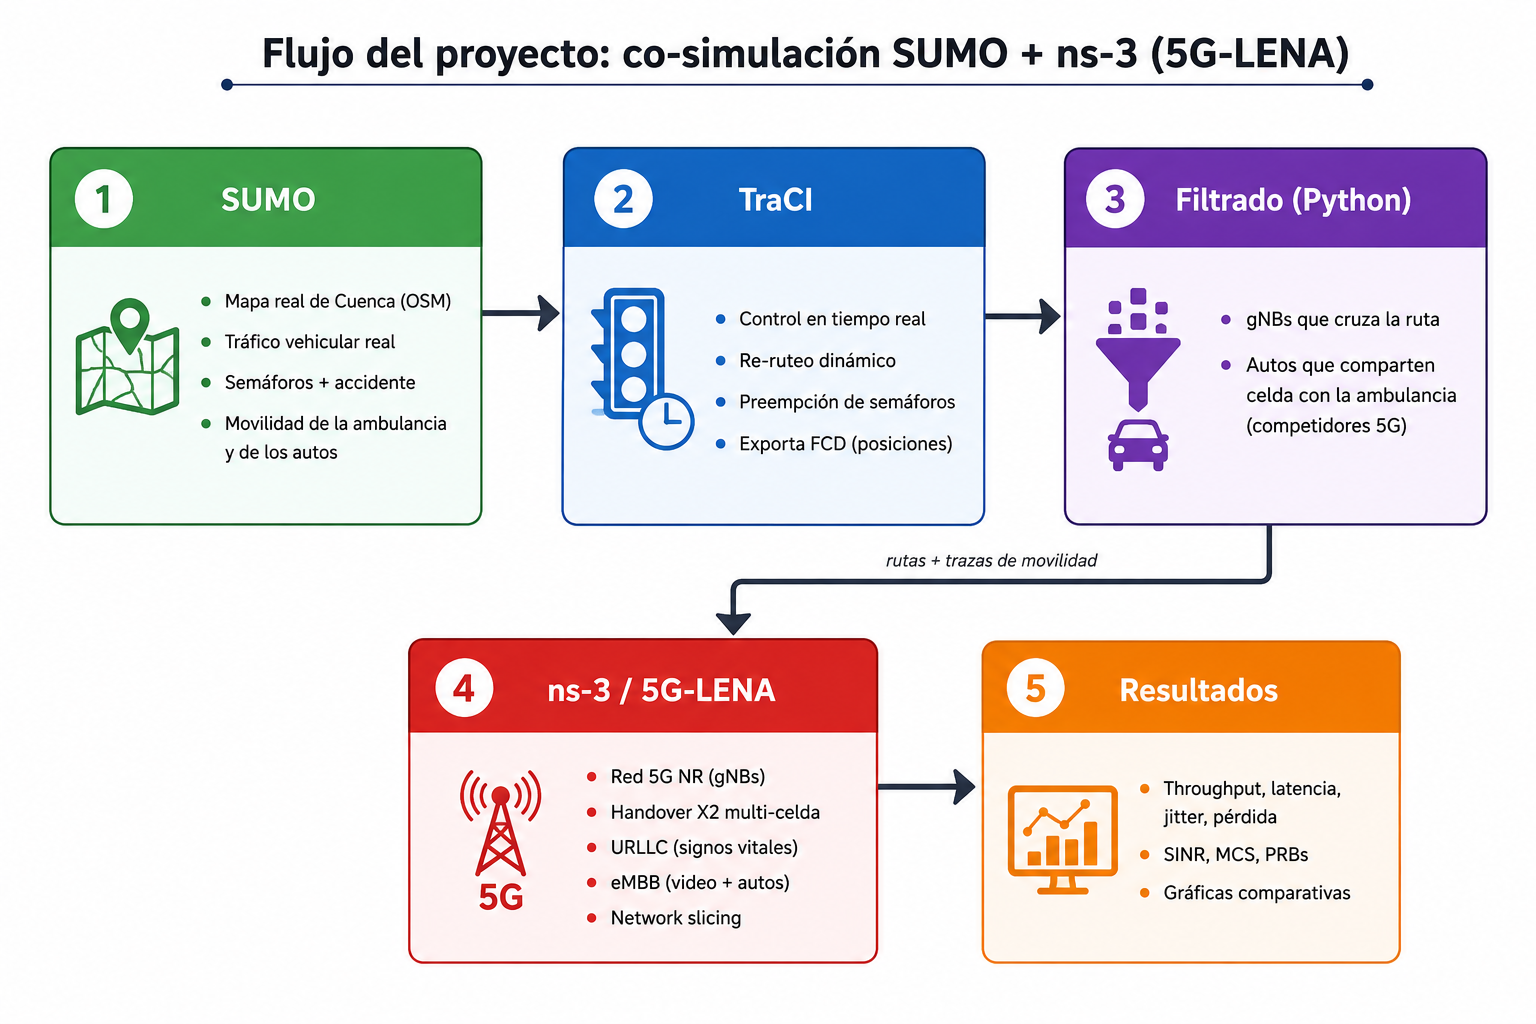
\includegraphics[width=\linewidth]{fig/diagrama_flujo.jpg}
\caption{Diagrama de bloques del flujo de la co-simulación: de la movilidad
vehicular (SUMO/TraCI) a la evaluación de la red 5G (ns-3/5G-LENA).}
\label{fig:flujo}
\end{figure}

\subsection{Escenario y herramientas}
Se descargó de OpenStreetMap el mapa real de Cuenca (una extensión de
$\approx 5.2\times4.7$~km) y se convirtió a una red vial de SUMO con 200
semáforos importados. Sobre ella se genera tráfico de fondo denso (miles de
vehículos con orígenes/destinos aleatorios) para reproducir condiciones de hora
pico. La Fig.~\ref{fig:sumo_ciudad} muestra una captura del entorno de
simulación de SUMO con el mapa y los edificios; la Fig.~\ref{fig:sumo_amb}
muestra un acercamiento con vehículos circulando (amarillos) y los semáforos en
las intersecciones. La ambulancia se modela como un vehículo de clase
\texttt{emergency} con dispositivo de sirena (\textit{bluelight}), ante el cual
el resto de conductores cede el paso.

\begin{figure}[H]
\centering
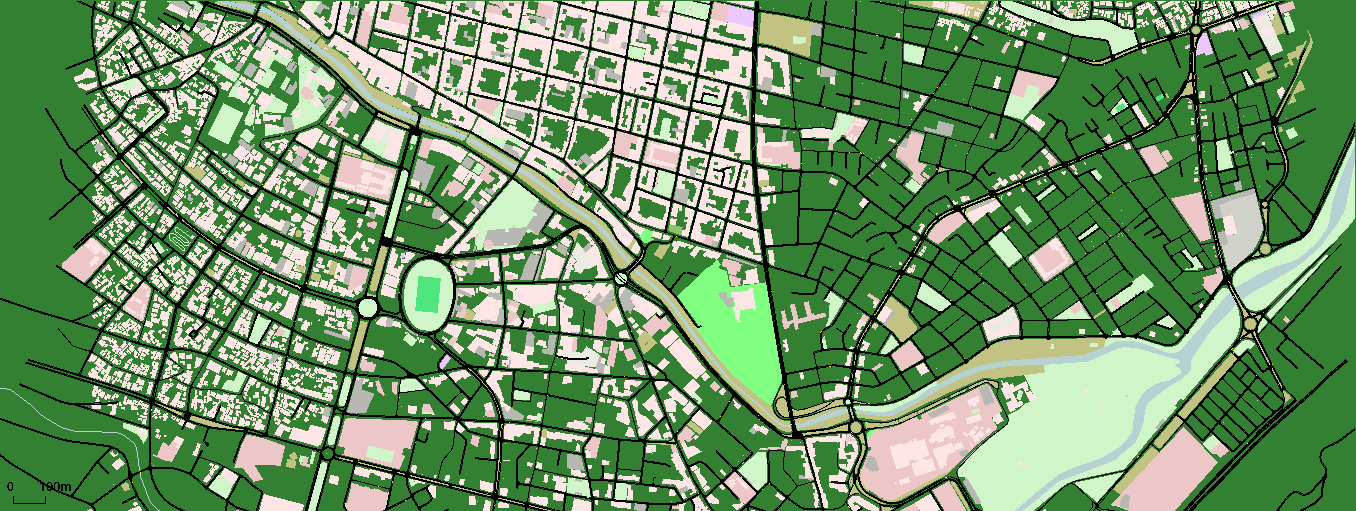
\includegraphics[width=\linewidth]{fig/01_trafico_ciudad.png}
\caption{Captura de SUMO: vista general del mapa real de Cuenca con edificios y
la red vial sobre la que circula el tráfico de fondo.}
\label{fig:sumo_ciudad}
\end{figure}

\begin{figure}[H]
\centering
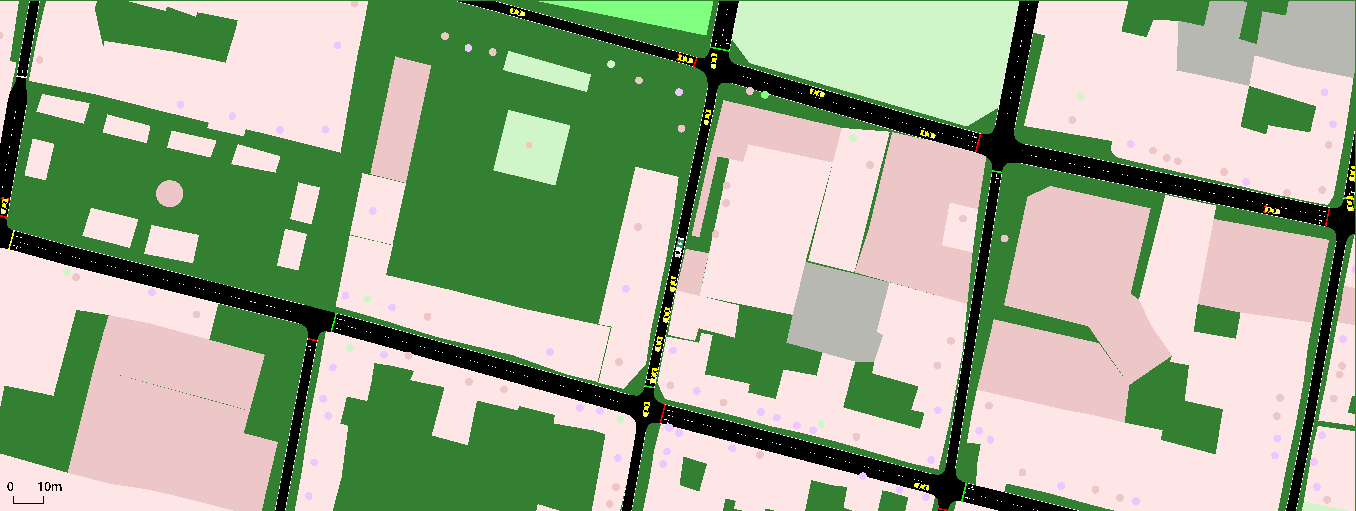
\includegraphics[width=\linewidth]{fig/02_ambulancia_trafico.png}
\caption{Captura de SUMO (acercamiento): vehículos circulando (rectángulos
amarillos) y semáforos en las intersecciones. La ambulancia, seguida por la
cámara, avanza entre el tráfico de la ciudad.}
\label{fig:sumo_amb}
\end{figure}

\subsection{Parámetros de la red 5G}
La Tabla~\ref{tab:params} recoge los parámetros de la red 5G NR simulada,
elegidos según los criterios de la asignatura de comunicaciones móviles: banda
FR1 de 3.5~GHz (banda n78), acceso OFDMA en modo TDD, modelo de propagación
Urban Macro (UMa) del 3GPP, y potencias de transmisión típicas de macrocelda.

\begin{table}[H]
\caption{Parámetros generales de la red 5G NR simulada.}
\label{tab:params}
\centering
\renewcommand{\arraystretch}{1.25}
\begin{tabular}{|l|l|}
\hline
\textbf{Parámetro} & \textbf{Valor} \\ \hline
Frecuencia portadora & 3.5 GHz (banda n78, FR1) \\ \hline
Ancho de banda & 10 -- 20 MHz \\ \hline
Numerología ($\mu$) & 1 (SCS 30 kHz) \\ \hline
Duplexación & TDD \\ \hline
Modelo de propagación & 3GPP Urban Macro (UMa) \\ \hline
Potencia Tx (gNB / UE) & 43 dBm / 23 dBm \\ \hline
Antenas (gNB / UE) & 4$\times$8 / 2$\times$4 (MIMO) \\ \hline
Planificador (\textit{scheduler}) & OFDMA Round-Robin \\ \hline
\textit{Slicing} / QoS & 2 \textit{bandwidth parts}: URLLC / eMBB \\ \hline
\textit{Handover} & X2 (multi-celda) \\ \hline
Núcleo de red & EPC (5G-LENA) \\ \hline
\textit{Bearers} & URLLC = DGBR ; eMBB = NGBR \\ \hline
\end{tabular}
\end{table}

\subsection{Fases de la metodología}
El trabajo se organiza en cuatro partes, alineadas con los paradigmas de 5G:

\textbf{Parte 1 -- mMTC (ruta dinámica y semáforos).} Mediante TraCI se
consideran todos los vehículos en tiempo real para: (a) recalcular
dinámicamente la ruta de menor tiempo de la ambulancia según el tráfico
existente, y (b) poner en verde los semáforos de su ruta (preempción). Se
inyecta además un accidente que bloquea una calle y obliga a re-rutear.

\textbf{Parte 2 -- Cobertura y filtrado (generación de tráfico 5G).} Se despliega
una red de 35 gNB que cubre toda la ciudad. Con la ruta ya calculada, se
identifican las gNB que atraviesa la ambulancia (intersección de la ruta con las
áreas de cobertura) y, dentro de ellas, los autos que comparten celda con la
ambulancia en los mismos instantes: los \textit{competidores} por recursos de
radio.

\textbf{Parte 3 -- Simulación 5G en ns-3.} Las trazas de movilidad de la
ambulancia y de los competidores filtrados alimentan ns-3/5G-LENA, donde se
genera el tráfico real de la red.

\textbf{Parte 4 -- URLLC + eMBB.} Se evalúa la coexistencia del tráfico crítico
y de banda ancha bajo carga, con y sin \textit{network slicing}.

\subsection{Adaptaciones al módulo 5G-LENA}
El módulo 5G-LENA (versión NR-v2.6) no soporta oficialmente el \textit{handover}
NR. Para el escenario multi-celda fue necesario portar y corregir la cadena de
señalización de traspaso heredada del módulo LTE (preparación por X2, orden RRC,
acceso aleatorio sin contención, conmutación de ruta y borrado de contexto),
además de tolerar la interrupción de datos que se produce en el instante del
traspaso cuando la celda está cargada. El estudio de carga (Parte 4) se realiza
sobre una única celda, aislando el fenómeno de contención sin \textit{handover}.

\section{Evaluación -- Análisis de resultados}

\subsection{mMTC: ruta dinámica, accidente y continuidad 5G}
La Fig.~\ref{fig:mapa1} muestra la ruta que la ambulancia sigue realmente,
generada por SUMO+TraCI, junto con la posición del accidente y las gNB 5G que la
sirven a lo largo del trayecto. Al detectar el accidente (Fig.~\ref{fig:acc},
captura de SUMO con el marcador rojo sobre la calle bloqueada), el servidor de
control recalcula la ruta y desvía a la ambulancia por calles libres. Es una
aplicación directa del paradigma mMTC: la decisión de ruteo se toma con
información de \textit{todos} los vehículos de la ciudad, en tiempo real.

\begin{figure}[H]
\centering
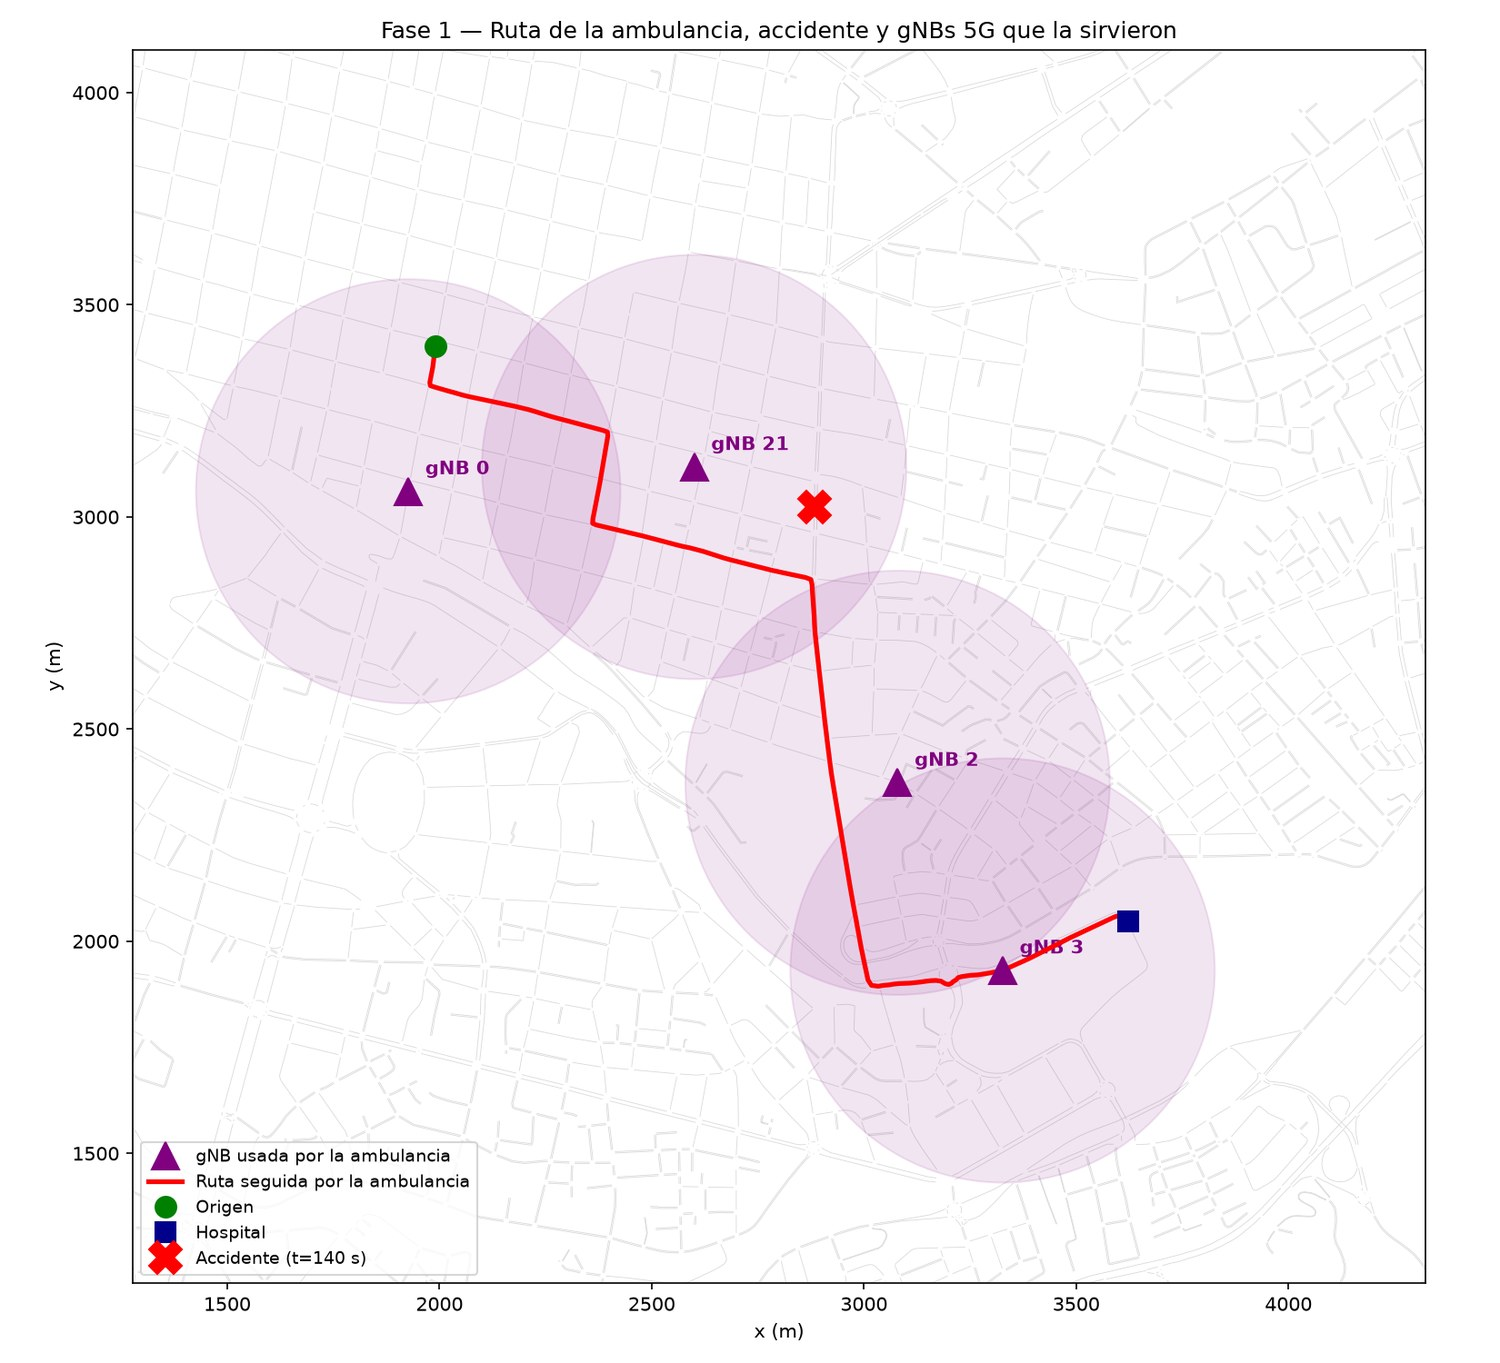
\includegraphics[width=0.92\linewidth]{fig/mapa1.jpg}
\caption{Ruta seguida por la ambulancia (roja) generada por SUMO+TraCI con
tráfico real y un accidente; los triángulos marcan las gNB 5G que la sirven y
sus áreas de cobertura.}
\label{fig:mapa1}
\end{figure}

\begin{figure}[H]
\centering
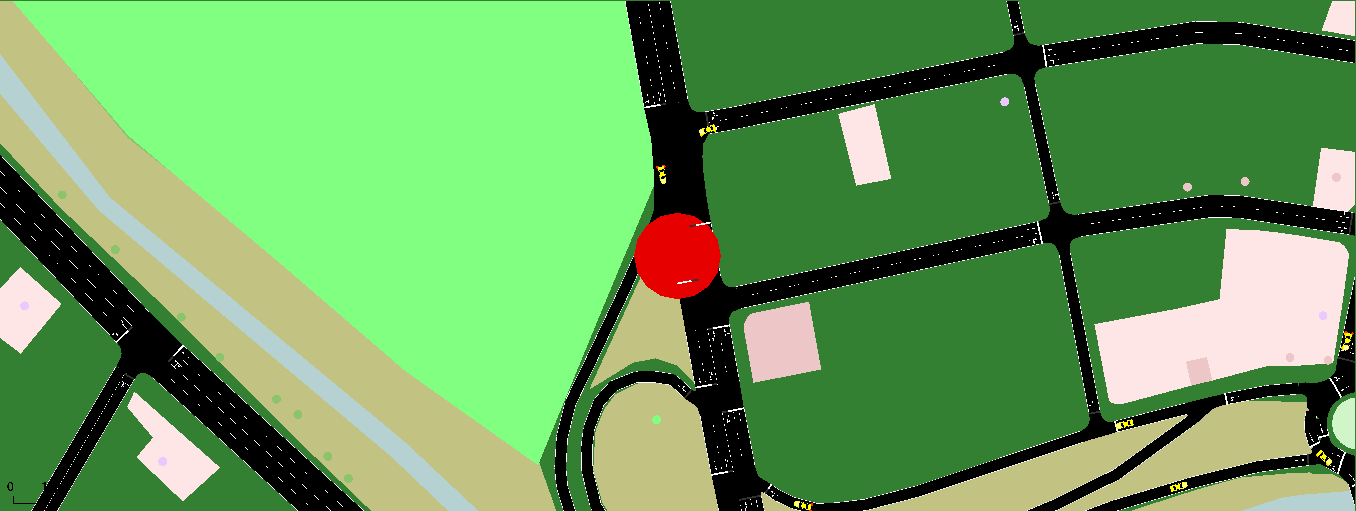
\includegraphics[width=\linewidth]{fig/03_accidente.png}
\caption{Captura de SUMO: indicador visual del accidente (marcador rojo) sobre
la calle bloqueada. El tráfico se detiene y la ambulancia es re-ruteada para
esquivarlo.}
\label{fig:acc}
\end{figure}

Desde el punto de vista de la red, la continuidad del servicio durante el
desplazamiento se evalúa con el SINR (\textit{Signal-to-Interference-plus-Noise
Ratio}). La Fig.~\ref{fig:sinr} presenta el SINR de control en el enlace
descendente frente al tiempo, junto con la distancia de la ambulancia a la gNB
más cercana. Gracias al despliegue multi-celda y al \textit{handover}, el SINR
se mantiene en valores útiles (no cae a cero) durante todo el recorrido: cada
vez que la ambulancia se aleja de una celda, el traspaso a la celda vecina evita
la pérdida de conexión. Las líneas verticales marcan los instantes de
\textit{handover}.

\begin{figure}[H]
\centering
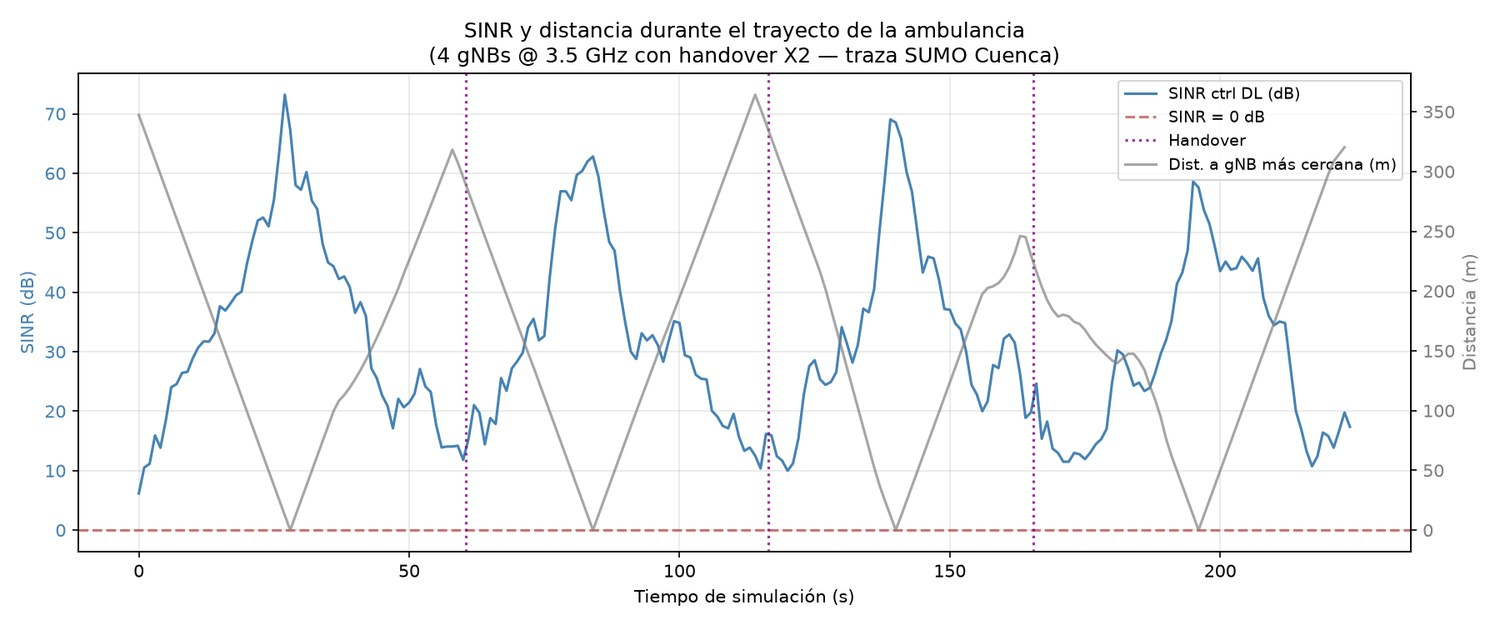
\includegraphics[width=\linewidth]{fig/sinr.jpg}
\caption{SINR de control (enlace descendente) y distancia a la gNB más cercana
en función del tiempo. Los \textit{handover} (líneas verticales) mantienen la
conexión al pasar de una celda a otra.}
\label{fig:sinr}
\end{figure}

El efecto de la asistencia 5G sobre el desempeño de la misión se resume en la
Fig.~\ref{fig:sistema}, que compara el tiempo de viaje, el tiempo detenida y el
número de detenciones de la ambulancia en hora pico para cuatro configuraciones:
sin asistencia, solo preempción de semáforos, solo re-ruteo dinámico, y el
sistema completo. El re-ruteo dinámico ---posible gracias al conocimiento en
tiempo real del tráfico--- es el componente dominante, y el sistema completo
reduce sustancialmente el tiempo de viaje frente al caso sin asistencia.

\begin{figure}[H]
\centering
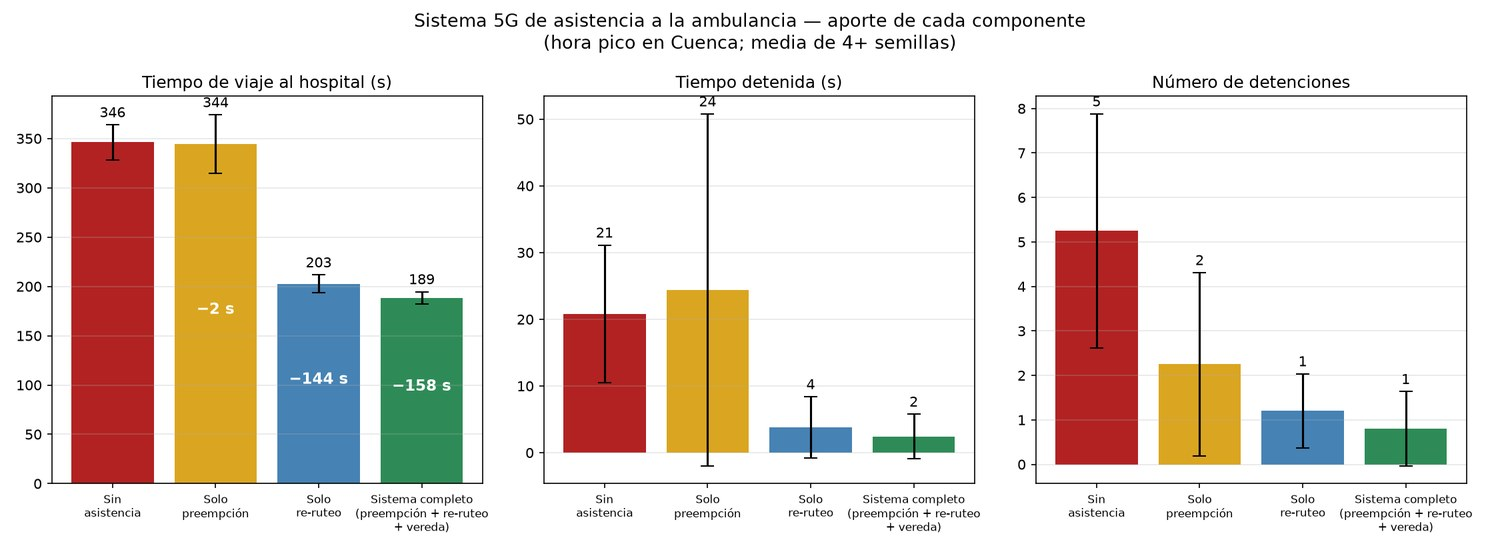
\includegraphics[width=\linewidth]{fig/sistema.jpg}
\caption{Aporte de cada componente de la asistencia 5G (preempción de semáforos,
re-ruteo dinámico, subida a la vereda) al tiempo de viaje, el tiempo detenida y
el número de detenciones de la ambulancia en hora pico.}
\label{fig:sistema}
\end{figure}

\subsection{Generación de tráfico 5G: cobertura y filtrado}
Para que el tráfico de red sea realista es necesario saber \textit{qué} autos
compiten por los recursos radio de la ambulancia. La Fig.~\ref{fig:cobertura}
muestra el despliegue de 35 gNB (rejilla hexagonal) que cubre toda la ciudad con
radio de buen servicio de $\approx$500~m a 3.5~GHz. Sobre este despliegue se
filtran, primero, las gNB por las que pasa la ambulancia como la intersección de
su ruta con las áreas de cobertura; y después, los autos cuya celda servidora
(la gNB más cercana) coincide con la de la ambulancia en los mismos instantes.

\begin{figure}[H]
\centering
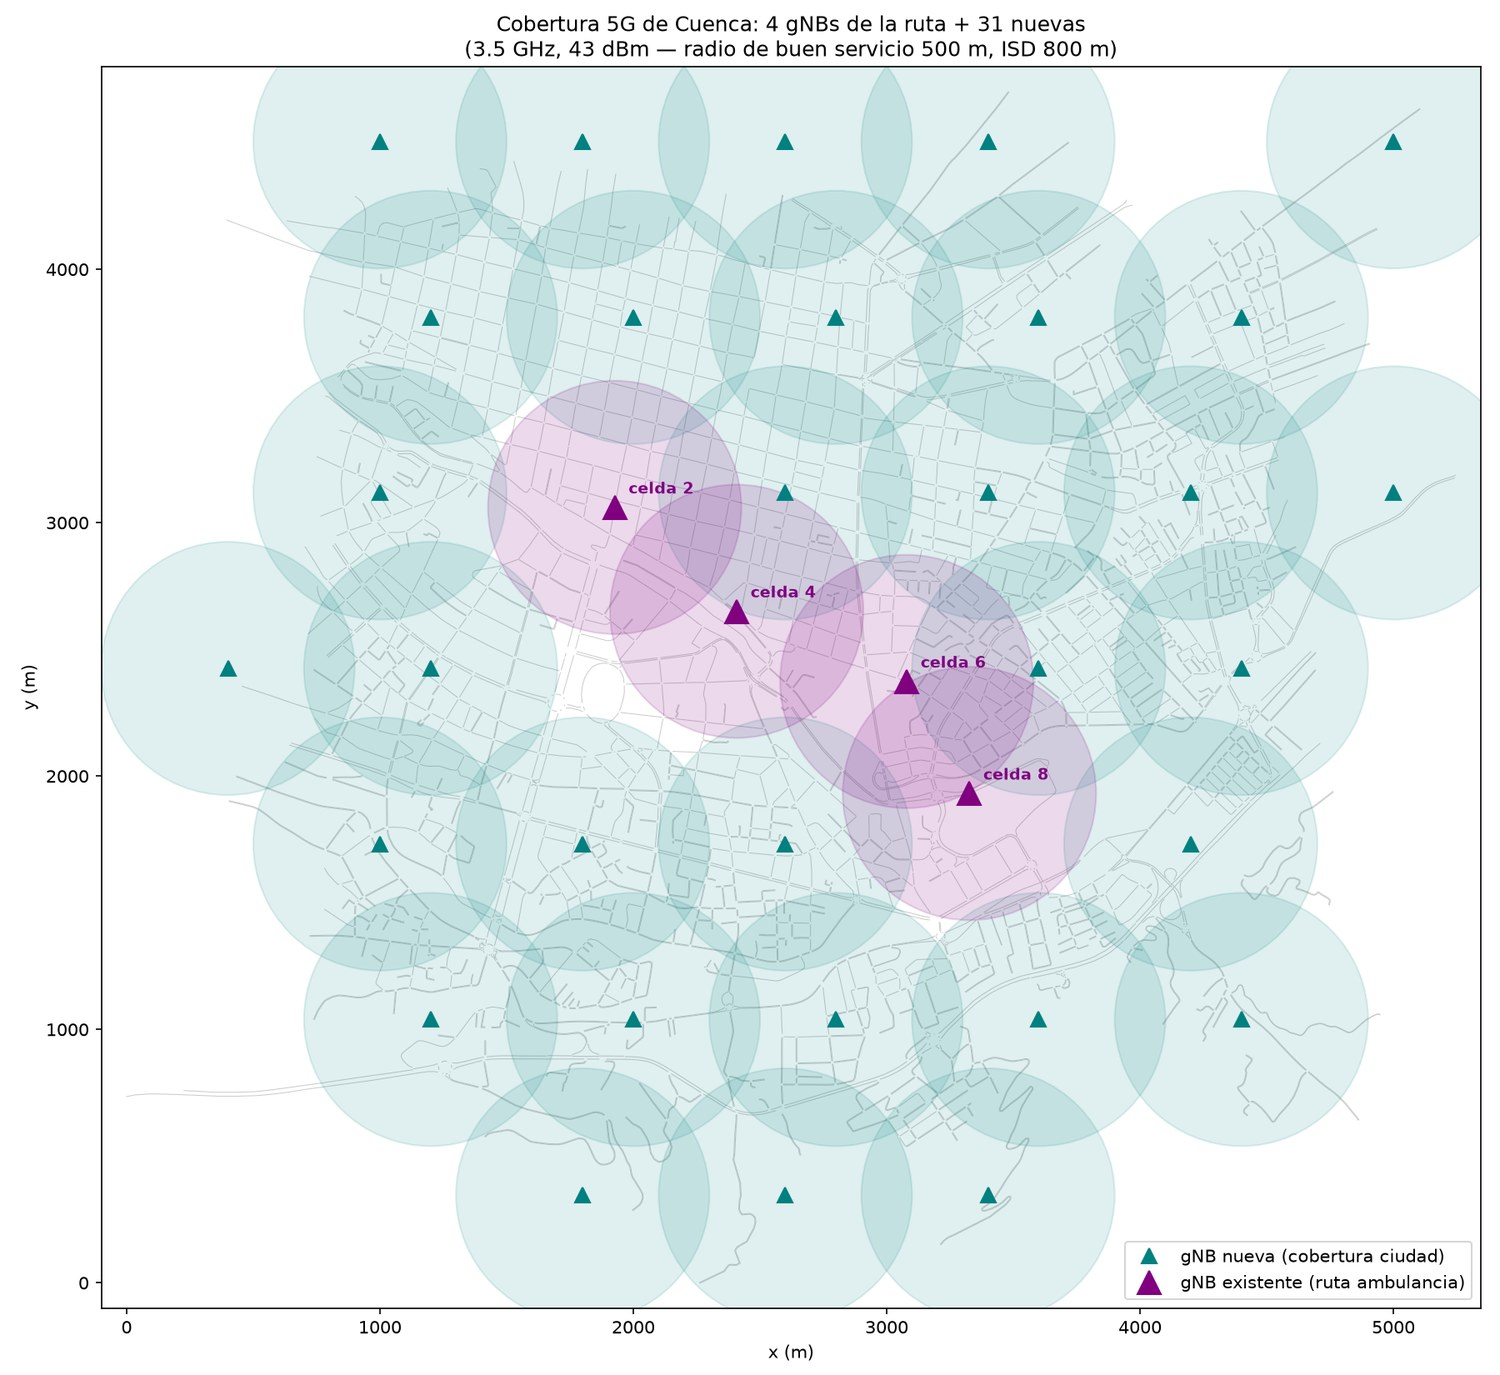
\includegraphics[width=0.9\linewidth]{fig/cobertura.jpg}
\caption{Despliegue de cobertura 5G sobre Cuenca: 4 gNB de la ruta (moradas) más
31 gNB adicionales (verdes) con sus áreas de servicio de $\approx$500~m. Sirve de
criterio para filtrar las celdas que atraviesa la ambulancia.}
\label{fig:cobertura}
\end{figure}

El resultado del filtrado se ilustra en la Fig.~\ref{fig:competidores}: en trazo
turquesa aparecen las trayectorias de los autos que compartieron celda con la
ambulancia (los competidores por recursos de radio), concentradas dentro de las
celdas de la ruta. Son estas trayectorias, y no un tráfico artificial, las que se
reproducen luego en ns-3 para cargar la red.

\begin{figure}[H]
\centering
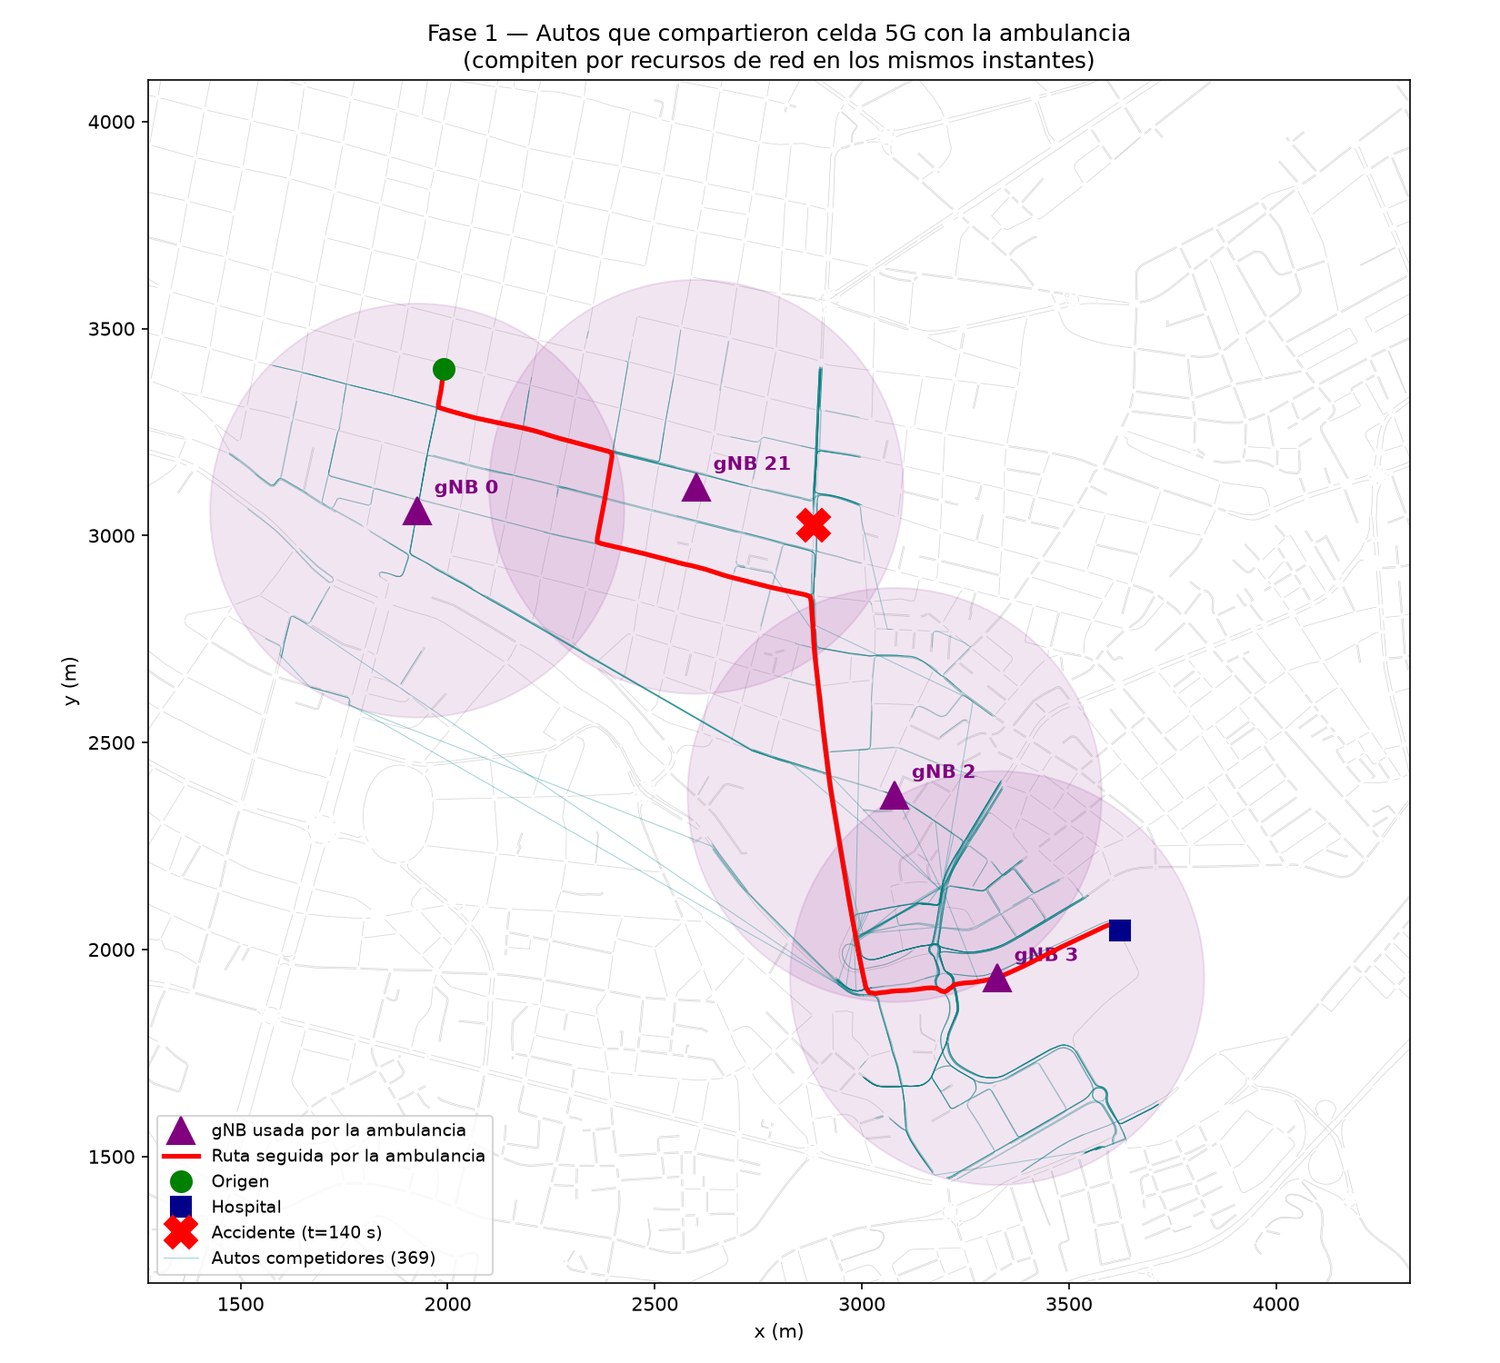
\includegraphics[width=0.9\linewidth]{fig/competidores.jpg}
\caption{Autos que compartieron celda 5G con la ambulancia en los mismos
instantes (competidores por recursos de radio). Sus rutas generan el tráfico de
carga en ns-3.}
\label{fig:competidores}
\end{figure}

\subsection{URLLC + eMBB bajo carga y \textit{network slicing}}
La ambulancia transmite al servidor del hospital dos flujos: signos vitales
(URLLC) y video (eMBB). Para evaluar su coexistencia se realizaron tres
simulaciones en ns-3 sobre una única celda cargada por los autos filtrados: (1)
solo el tráfico de la ambulancia (sin carga); (2) ambulancia + autos, sin
\textit{slicing} (todo el tráfico comparte una banda de 10~MHz); y (3)
ambulancia + autos, con \textit{slicing} (el espectro se parte en una banda
dedicada de 2~MHz para URLLC y 8~MHz para eMBB). Es importante notar que el video
de la ambulancia y el tráfico de los autos son \textbf{ambos} tráfico eMBB.

La Fig.~\ref{fig:fase3} presenta las métricas resultantes (latencia, jitter,
pérdida y throughput) para los flujos de la ambulancia en las tres
configuraciones. Sin carga (izquierda) ambos flujos se entregan sin pérdida.
\textbf{Con carga y sin \textit{slicing}}, la celda se satura y se pierde el
100\,\% del tráfico crítico URLLC (los signos vitales no llegan). \textbf{Con
carga y con \textit{slicing}}, en cambio, los signos vitales se entregan
\textit{intactos} (0\,\% de pérdida, $\approx$7~ms de latencia), porque viajan en
una banda de espectro físicamente separada que el tráfico eMBB no puede tocar; el
precio es que el tráfico eMBB (video + autos), que excede la capacidad de su
banda, se sacrifica. Este es el resultado central del trabajo: el
\textit{slicing} no crea capacidad, sino que \textbf{decide a quién proteger}
cuando la red se congestiona, garantizando el servicio de misión crítica.

\begin{figure}[H]
\centering
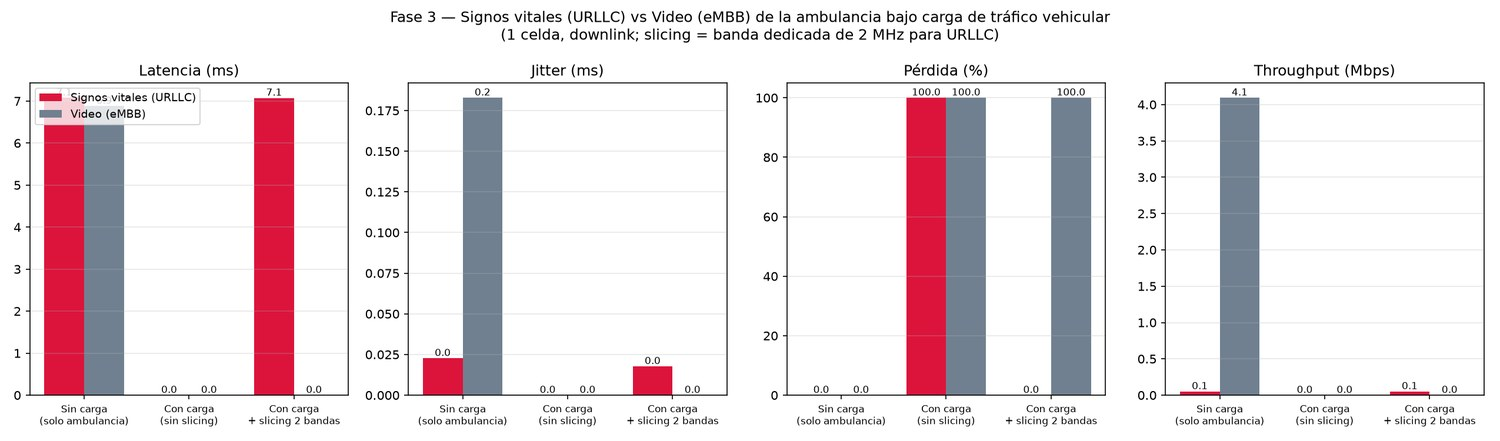
\includegraphics[width=\linewidth]{fig/fase3.jpg}
\caption{URLLC (signos vitales) vs. eMBB (video) de la ambulancia bajo carga
vehicular. El panel de pérdida es determinante: sin \textit{slicing} se pierde el
100\,\% del tráfico crítico; con \textit{slicing}, 0\,\%.}
\label{fig:fase3}
\end{figure}

\subsection{Comportamiento del planificador (\textit{scheduler})}
Para explicar \textit{cómo} se reparten los recursos, se instrumentó el
planificador OFDMA Round-Robin. La Fig.~\ref{fig:sched_thr} muestra el throughput
entregado a cada flujo a lo largo del tiempo (áreas apiladas). Sin carga, la
ambulancia dispone de toda la celda; con carga, el Round-Robin reparte la celda
entre la ambulancia y los autos; y con \textit{slicing}, los signos vitales
(URLLC) ocupan una franja propia y aislada, separada del video (eMBB). La
Fig.~\ref{fig:sched_rep} muestra el reparto agregado de recursos: sin
\textit{slicing} el Round-Robin distribuye los recursos de forma
aproximadamente equitativa entre todos los usuarios, mientras que con
\textit{slicing} los signos vitales tienen su porción de espectro reservada,
independientemente de la carga eMBB.

\begin{figure}[H]
\centering
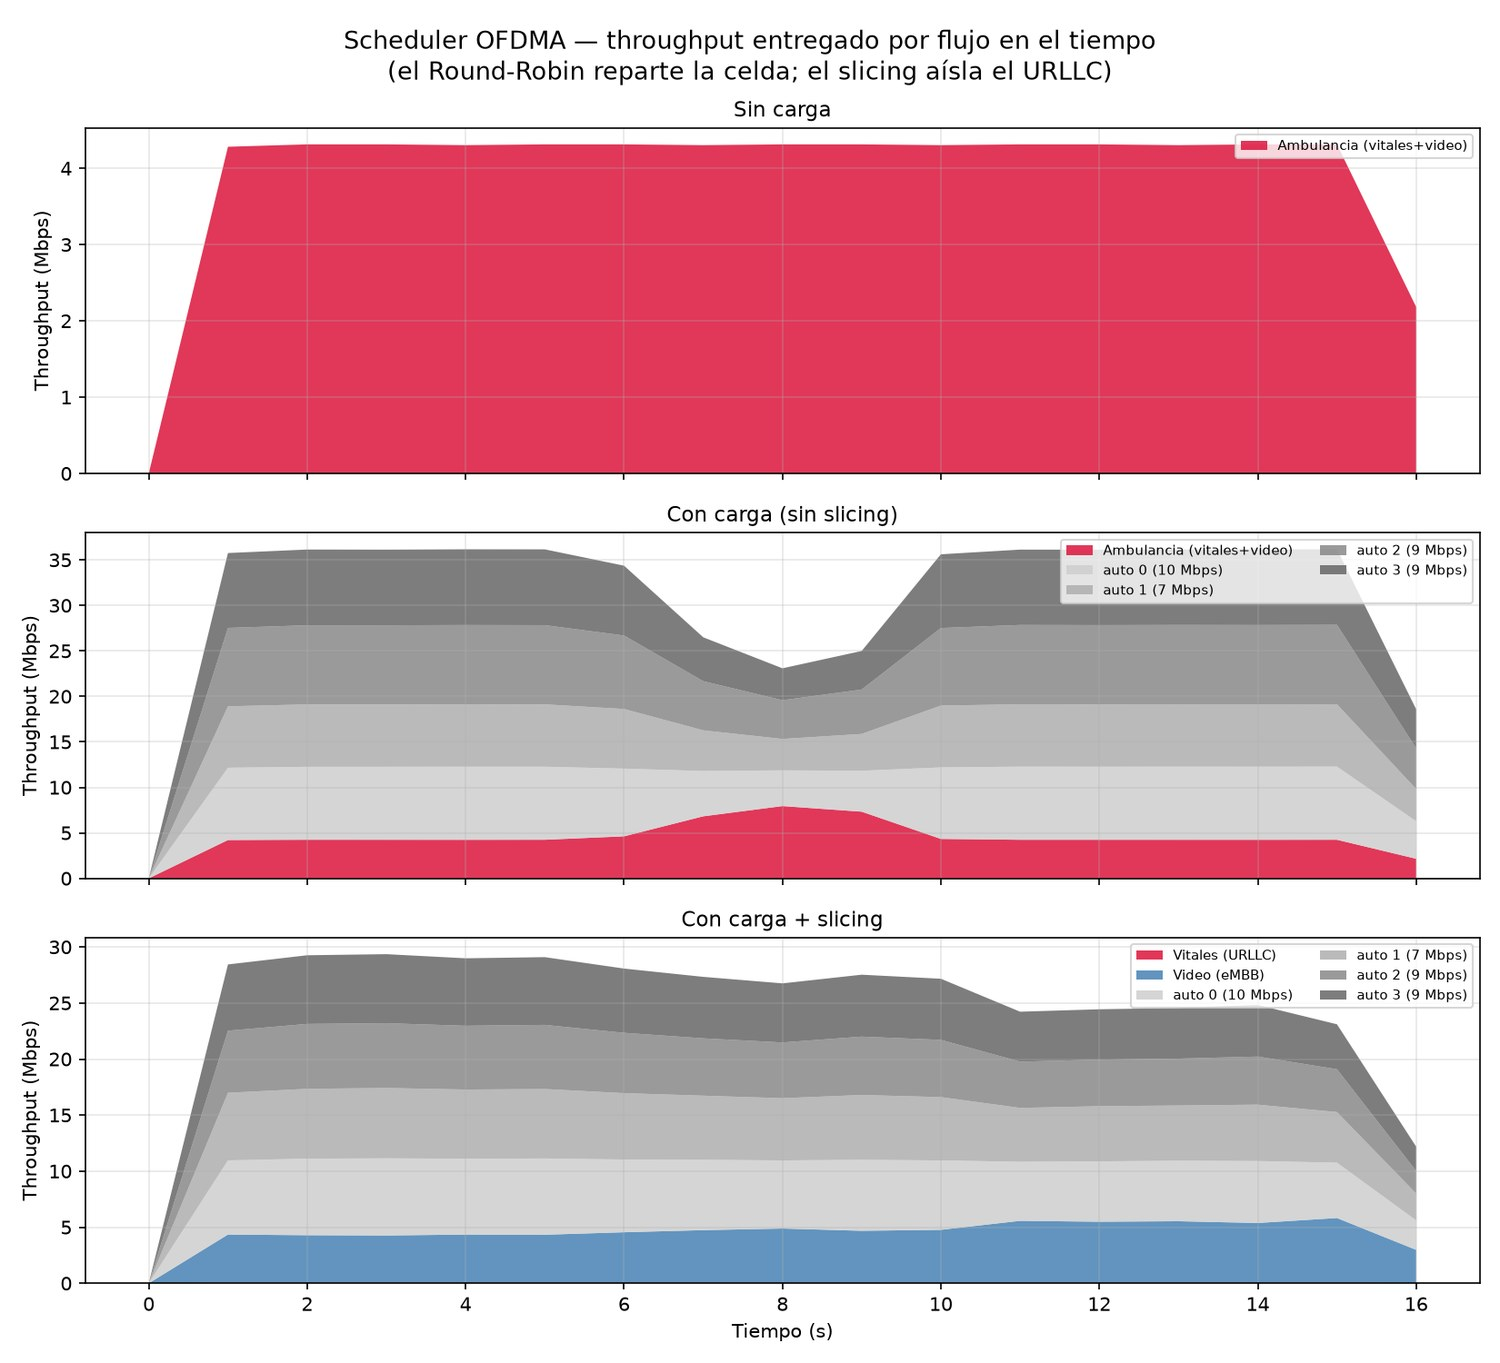
\includegraphics[width=\linewidth]{fig/sched_thr.jpg}
\caption{Planificador OFDMA: throughput entregado por flujo en el tiempo. Con
\textit{slicing}, los signos vitales (URLLC) ocupan una franja aislada,
protegida de la contención eMBB.}
\label{fig:sched_thr}
\end{figure}

\begin{figure}[H]
\centering
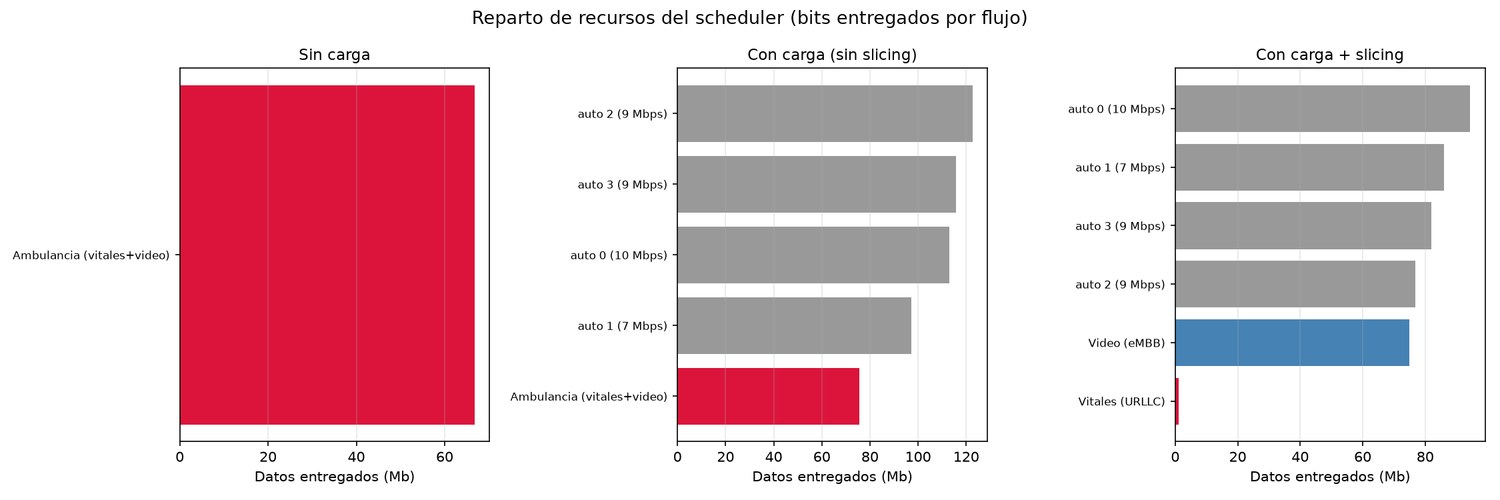
\includegraphics[width=\linewidth]{fig/sched_rep.jpg}
\caption{Reparto agregado de recursos del planificador por flujo. Sin
\textit{slicing} el reparto es equitativo entre todos; con \textit{slicing}, los
signos vitales tienen espectro reservado.}
\label{fig:sched_rep}
\end{figure}

\section{Conclusiones}
Se construyó y evaluó una co-simulación acoplada SUMO + ns-3/5G-LENA que modela,
sobre el mapa real de Cuenca, un caso de uso de misión crítica de 5G integrando
los paradigmas mMTC, URLLC y eMBB. Las principales conclusiones, desde la óptica
de comunicaciones móviles, son:

\begin{itemize}
\item El uso de información de \textit{todos} los vehículos en tiempo real (mMTC)
permite re-rutear dinámicamente a la ambulancia y sincronizar los semáforos,
reduciendo de forma notable el tiempo de viaje; el re-ruteo dinámico resultó ser
el componente más influyente.
\item El despliegue multi-celda con \textit{handover} X2 mantiene el SINR en
valores útiles a lo largo de toda la ruta, garantizando la continuidad del
servicio de la red móvil durante el desplazamiento.
\item El filtrado de los vehículos que comparten celda con la ambulancia, a
partir de un despliegue que cubre la ciudad, permite generar un tráfico de red
\textit{realista} en ns-3, en lugar de un tráfico sintético.
\item Bajo saturación de la celda, sin \textit{network slicing} el tráfico
crítico URLLC (signos vitales) se pierde por completo, mientras que con
\textit{slicing} por \textit{bandwidth part} se garantiza su entrega con 0\,\% de
pérdida y latencia de milisegundos, a costa del tráfico eMBB no crítico. El
\textit{slicing} es, por tanto, un mecanismo esencial para los servicios de
misión crítica en redes 5G congestionadas.
\item El análisis del planificador OFDMA evidencia que, sin diferenciación, un
reparto equitativo (Round-Robin) no basta para proteger el tráfico crítico
cuando la demanda supera la capacidad; la reserva de recursos (\textit{slicing})
es la que aporta la garantía.
\end{itemize}

El código, los datos y las instrucciones de reproducción están disponibles en el
repositorio público del proyecto~\cite{repo}:
\url{https://github.com/thyron001/ambulace5G}.

\bibliographystyle{IEEEtran}
\bibliography{referencias}

\end{document}
